\section{Theoretical Describtion of the functionality of a Laser}
\label{sec:theory}

A laser (Light Amplification by Emission of Radiation) comprises
three essential components. These components include a laser medium, 
which in this instance is a gas mixture of helium and neon, a pump
source, specifically an electric discharger and an optical resonator, 
in this case one partially and one fully reflecting mirror.

The laser medium is responsible for the laser's radiation spectrum, 
primarily due to its specific excitation energy. In the case 
of a HeNe laser, the active laser medium is the noble gas neon. 
This laser medium possesses various energy states, enabling three 
fundamental processes, as illustrated in Figure~\ref{fig:emission}.

If the atom is in the ground state, it can absorb a photon with
the requiered energy for excitation, resulting in the atom having 
one electron at a higher energy level. This process is known as 
absorption. An excited atom can spontaneously transition back 
to the lower energy groundstate, emitting a photon with the remaining 
energy, in line with energy conservation. The direction of the emitted
photon is random. This process is called spontaneous emission.
Another de-excitation process is stimulated emission. In this case
an excited atom is struck by a photon with precisely the same 
energy as the difference between the excited and ground state. 
This causes the atom to emit a photon and return to the ground state.
The incoming and emitted photons have the same energy, direction and 
phase, making them coherent.

\begin{figure}
    \centering
    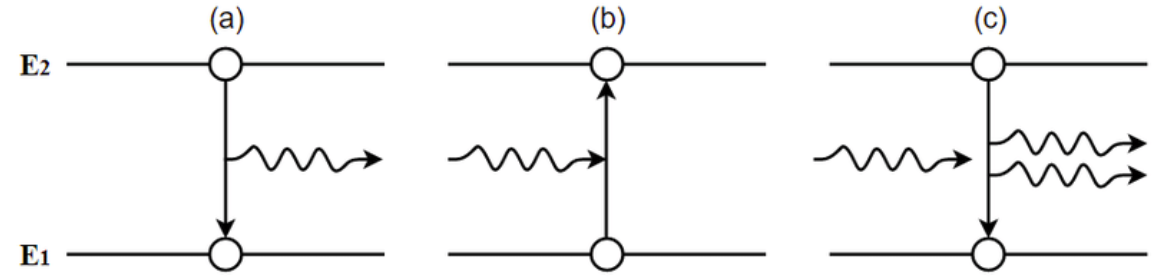
\includegraphics[width=0.8\linewidth]{pictures/emission.png} %https://www.researchgate.net/figure/a-Spontaneous-Emission-b-Stimulated-Absorption-c-Stimulated-Emission_fig2_335822340
    \caption{Diagrammatic representation of absorption (a), spontaneous emission (b), and stimulated emission (c) for a two-state system. \cite{emission}}
    \label{fig:emission}
\end{figure}

In contrast to the illustration in Figure \ref{fig:emission}, a laser 
requieres a laser medium with more than two energy levels. In a two 
level system, the Einstein coefficients $B_{12}$ and $B_{21}$, which 
describe the transition probability between states, are equal. Due to 
this, the population inversion necessary for the laser is not achievable
in a tow-level system.

To archieve population inversion, a pump source must input energy 
into the system. In the case of a HeNe laser, an electric discharger 
pumps energy into the pump gas helium. The excited helium atoms 
collide with neon atoms, transfering their energy. The level diagram is 
illustrated in Figure \ref{fig:level}.

\begin{figure}
    \centering
    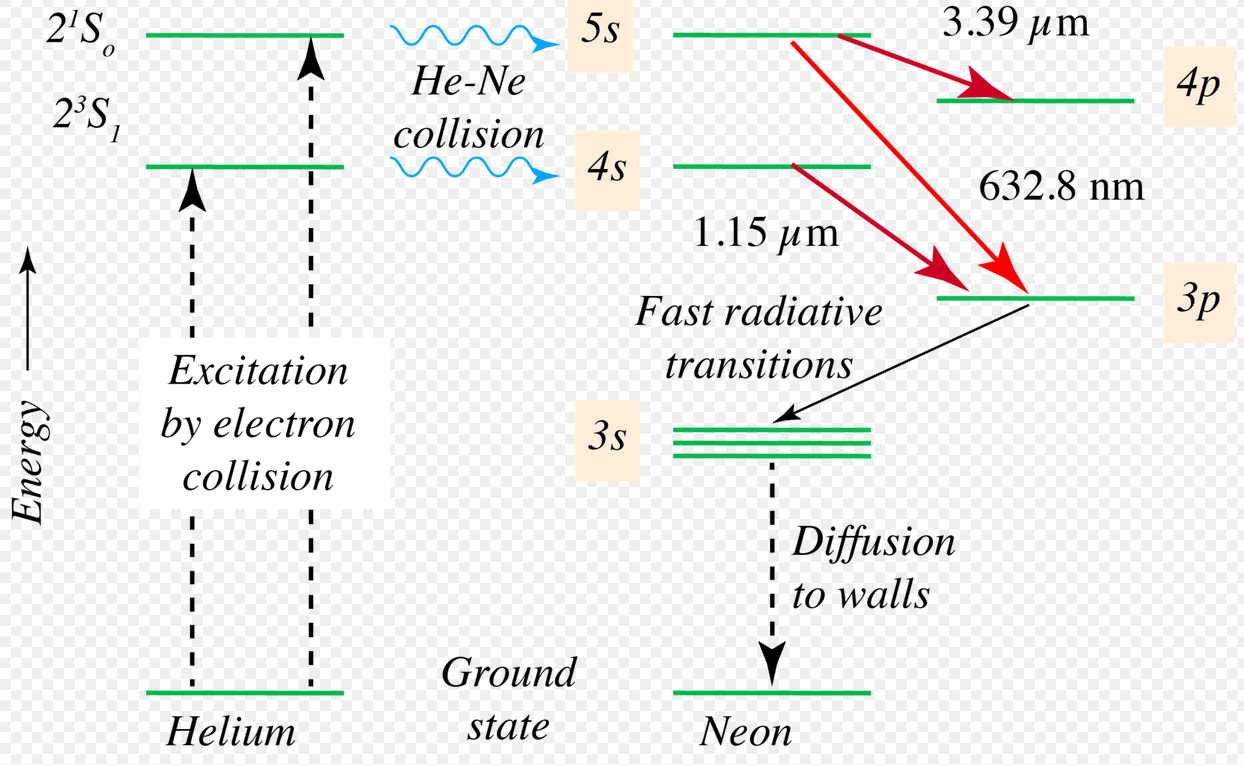
\includegraphics[width=0.7\linewidth]{pictures/level.png} %https://en.wikipedia.org/wiki/Helium%E2%80%93neon_laser
    \caption{Diagramtic representation of the level schema for the HeNe lasers. \cite{Wikipedia}}
    \label{fig:level}
\end{figure}
The transition from the 3s to the p2 state predominates the process, 
resulting in the production of red laserlight with a wavelength of 
$\lambda = \SI{632.8}{\nano\meter}$.

As amplification is dependent on the distence traveled, a resonator is 
employed to increase the pathlength. This is implemented using two 
mirrors, one fully reflecting and one partically reflecting, enabling
the beam to exit the laser tube in one direction.

To control the laser, the resonator must satisfy the stability relation
\begin{equation}
    0 < g_1g_2 \leq 1
    \label{eqn:stability}
\end{equation}

where $g_i=1-\frac{L}{r_i}$ is defined with the length $L$ and the 
curvature radius $r_i$ of the mirror $i$. If condition \eqref{eqn:stability}
is not met, the laser beam may grow until it becomes larger than the mirror,
resulting in its loss. Figure \ref{fig:resonator} displays two resonators,
one stable and one unstable.

\begin{figure}[H]
    \centering
    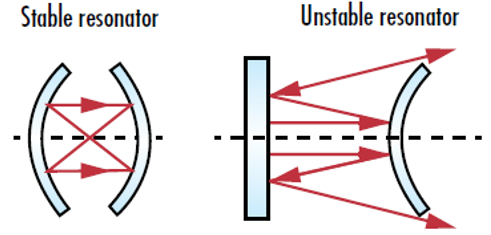
\includegraphics[scale=0.5]{pictures/resonator.png} %https://www.edmundoptics.de/knowledge-center/application-notes/lasers/laser-resonator-modes/
    \caption{Graphical illustration of the beam path in one resonator that fulfills the stability condition \eqref{eqn:stability} (left) and an unstable resonator (right). \cite{resonator}}
    \label{fig:resonator}
\end{figure}

The light forms standing waves between the mirrors, denoted as $\text{TEM}_{pl}$,
where $p$ and $l$ describe the radial and angular mode orders. Figure 
\ref{fig:TEM} shows the patterns of the first orders.

%\begin{figure}[H]
%    \centering
%    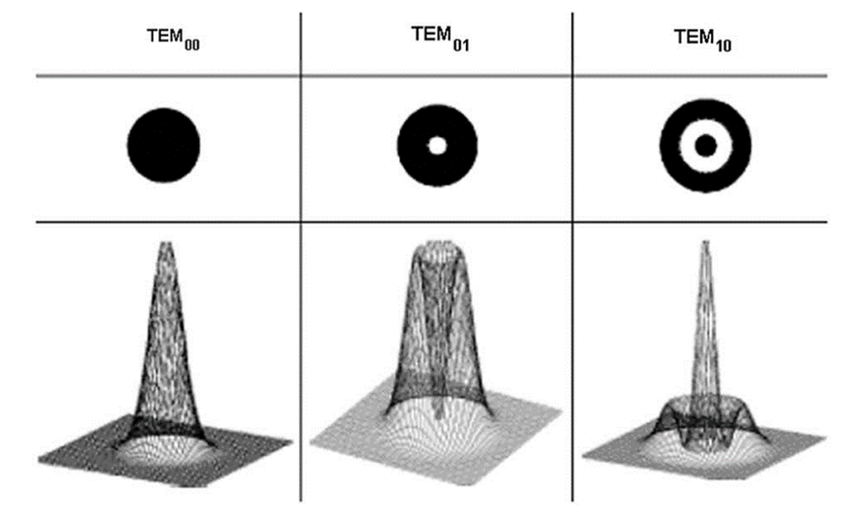
\includegraphics[scale=0.3]{pictures/modes.png} %https://www.researchgate.net/figure/Different-Transverse-electromagnetic-mode-for-lasers-19_fig8_321225714
%    \caption{The intensity distribution of the laser modes $\text{TEM}_{00}$, $\text{TEM}_{01}$ and $\text{TEM}_{10}$. \cite{TEM}}
%    \label{fig:TEM}
%\end{figure}
\begin{figure}[H]
    \centering
    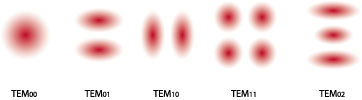
\includegraphics[scale=0.8]{pictures/modes2.jpg} %https://www.researchgate.net/figure/Different-Transverse-electromagnetic-mode-for-lasers-19_fig8_321225714
    \caption{The intensity distribution of the laser modes $\text{TEM}_{00}$, $\text{TEM}_{01}$, $\text{TEM}_{10}$, $\text{TEM}_{11}$ and $\text{TEM}_{02}$. \cite{TEM2}}
    \label{fig:TEM}
\end{figure}

It can be observed that the ground mode $\text{TEM}_{00}$ follows a 
Gaussian distribution, which can be described in polar corrdonates by:

\begin{equation}
    I(r)=I_0 \exp{\left(\frac{-2r^2}{\omega^2}\right)}.
\end{equation}
